\section{Metodología}
\subsection{Diseño, procedencia y separación de evidencia}
El estudio es computacional, cuantitativo y experimental, con evaluación cronológica de origen móvil. La descripción del error corresponde a servicio, recurso, condición, inicialización y realización de máscara. Las ventanas se solapan y los servicios comparten infraestructura. Una fila de resultados no equivale a una réplica independiente. La fase histórica es exploratoria; el escenario principal ampliado contiene cuatro contrastes preespecificados localmente. Los restantes análisis se presentan descriptivamente. La Tabla~\ref{tab:master} relaciona sus unidades y presupuestos.

El histórico contiene 8005 filas temporales compartidas, dos recursos y 28 servicios, con historia 12 y horizonte de un paso, equivalente a treinta minutos. Utiliza tres semillas, veinte máscaras y siete condiciones: datos completos y pérdidas dispersas o por bloques de 10, 20 y 40\%. Se conservan E0--E5, C0--C3, V2 y comparadores originales. V2 selecciona una familia compacta entrenada mediante validación; no es un modelo ajustado de forma independiente. La auditoría comprueba manifiestos y archivos preservados. No se combinan sus errores con los nuevos como si fueran repeticiones independientes.

ChronoGraph publica series nominalmente semihorarias y relaciones de llamadas \cite{chronograph}. El grafo publicado contiene 708 servicios y 1529 aristas. Los subconjuntos analizados no implican ajustar sobre los 708 servicios. Los cortes son $[0, 5603)$, $[5603, 6404)$ y $[6404, 8005)$:70/10/20 por filas, con redondeo. Existe un salto de 108000 segundos después de la fila 5907, dentro de validación. Ventanas y pares consecutivos del denominador MASE no atraviesan ese hueco. Para L12/H1 existen 5591 orígenes de entrenamiento, 777 de validación y 1589 de prueba históricos. La cohorte fuente es de conveniencia; el subgrafo histórico conserva 28 aristas internas y excluye 137 de frontera según la auditoría.

La cohorte destino de 32 servicios se elige mediante topología estática y recorrido reproducible ordenado por SHA, excluyendo los 28 originales y cuatro pilotos conocidos. No utiliza errores predictivos. Su conexión topológica y selección de conveniencia limitan la representatividad poblacional. Los pesos e hiperparámetros usan solo entrenamiento/validación fuente. Para cada servicio destino, sus primeras 5603 filas aportan media, desviación, mediana y denominador MASE. La validación destino no selecciona modelos. Se trata de transferencia espacial calibrada, no de pronóstico sin datos previos del destino. La CPU conserva la escala publicada y la memoria se mide en bytes; no se convierte CPU arbitrariamente a porcentaje o núcleos. El modelo de grafo recibe nuevas matrices de adyacencia, sin aprender pesos destino. No se estableció completamente la fecha de disponibilidad de cada arista.

El caso externo utiliza los primeros 48 objetos oficiales \texttt{MSMetricsUpdate} de Alibaba 2022, correspondientes a un día \cite{alibaba2022}. Una cola limitada verifica Content-MD5 del propietario y registra SHA256. Se descargaron 17890753336 bytes con 675424445 filas CSV de pods. Entre los servicios con cobertura de todos los instantes del primer objeto se eligen 32 por orden SHA y se ordenan lexicográficamente. La selección atiende a disponibilidad, no a precisión. Para cada instante se promedian pods por servicio con ambos recursos finitos; después se promedian esos instantes con el mismo peso dentro del intervalo semihorario. Un intervalo con menos de treinta observaciones de minuto válidas se considera ausente y solo queda disponible al cierre.

Alibaba publica utilización normalizada min--max, no núcleos ni bytes. El alcance temporal de esa normalización no está documentado aquí. Los 48 intervalos procesados se dividen en 12 de calibración, seis horas, y 36 objetivos, dieciocho horas. Cuatro valores escalares naturalmente ausentes se encuentran solo en calibración, dos pares servicio/intervalo en ambos recursos. Ningún objetivo externo se imputa. Los pesos fuente L12/H1 permanecen congelados, sin ajuste ni selección externa. Se excluye GRU de grafo porque no se adquirió la red de llamadas externa. Este diseño no aplica 70/10/20 a Alibaba y constituye un caso exploratorio corto.

\subsection{Preparación causal, normalización y máscaras}
Sea $ y_{t,s,r}$ la medición de recurso $ r $, servicio $ s $ e instante $ t $. Cada recurso se pronostica por separado. Una entrada de $ L $ pasos termina en $ t-h $ y produce directamente el objetivo $ y_{t,s,r}$. Los límites de partición y huecos reinician la preparación. Se calcula $ x=(y-\mu)/\max(\sigma, 10^{-8})$ con estadísticas del prefijo correspondiente; la inversión devuelve $\widehat y=\sigma_*\widehat x+\mu $. Las estadísticas de calibración preceden las máscaras sintéticas. Por ello no se evalúa aprender esas estadísticas a partir de un prefijo artificialmente degradado.

Una medición disponible se conserva; cuando falta, se arrastra la última observación del segmento y, antes de la primera, se usa la mediana de entrenamiento. El indicador observado es $ m $, el de ausencia después de observar es $ c $ y el de respaldo por mediana es $ f $, con $ m+c+f=1$. La edad satisface $\delta_i=(1-m_i)(\delta_{i-1}+1)$ y comienza en cero antes del segmento. Si no hubo observación dentro de este, mide la racha desde el corte, no un tiempo real desconocido anterior. Los canales contienen valor normalizado preparado, $ m $, edad $\log(1+\delta)/\log(1+L)$, $ c $ y $ f $. El arrastre y la edad pueden resumir una observación anterior a la ventana explícita; $ L $ no limita estrictamente toda la información histórica.

Las siete condiciones originales conservan cantidades redondeadas exactas de ausencias por servicio y segmento. El patrón disperso selecciona entradas; el de bloques usa candidatos de hasta seis pasos. Se comparten máscaras entre métodos y recursos, y los objetivos originales permanecen disponibles para evaluación. El caso completo se cuenta una vez. Las tasas históricas son anidadas. Tres condiciones adicionales con etiqueta nominal 20\% incluyen pérdidas correlacionadas en grupos consecutivos de ocho servicios lexicográficos, bloques prolongados candidatos de hasta 24 pasos y MAR dependiente del retardo. La construcción de bloques deja separadores y puede truncar el último bloque para alcanzar el conteo exacto. Estas estructuras se imponen; no son interrupciones registradas.

La probabilidad MAR implementada es
\begin{equation}
 p_t=0.2\{1+0.5\tanh(|z^{\mathrm{CPU,ultima}}_t|)\},
\end{equation}
donde $ z^{\mathrm{CPU,ultima}}_t $ utiliza exclusivamente CPU observada previamente. Por tanto,$0.2\leq p_t<0.3$:20\% es una etiqueta nominal. La máscara compartida se intersecta con disponibilidad natural. El principal utiliza veinte semillas de máscara emparejadas entre modelos y entrenamientos. Esa secuencia se había usado históricamente; cambiar de servicios no la convierte en inédita. Las Figs.~\ref{fig:masks} y~\ref{fig:temporal} muestran los mecanismos y la preparación temporal.

\begin{figure*}[t]\centering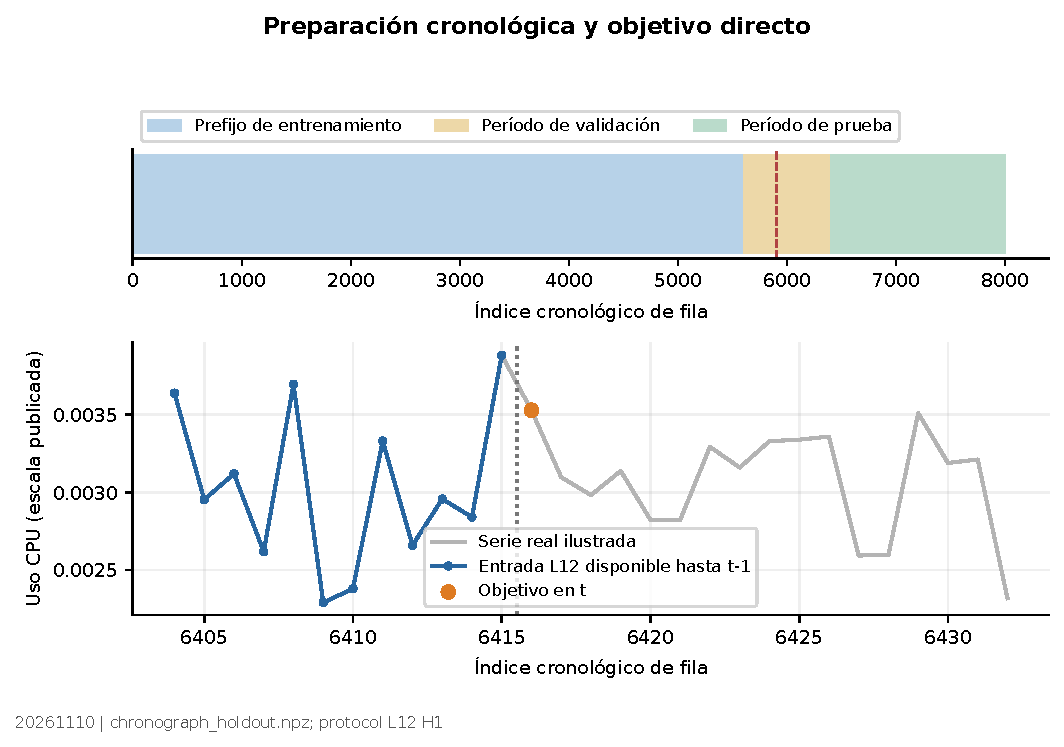
\includegraphics[width=0.72\textwidth]{figuras/es_04_temporal_preparation.pdf}
\caption{Cortes por filas y hueco de validación después de 5907. El ejemplo inferior usa valores reales L12/H1; el contexto posterior gris queda excluido de la entrada.}\label{fig:temporal}\end{figure*}

\begin{figure*}[t]\centering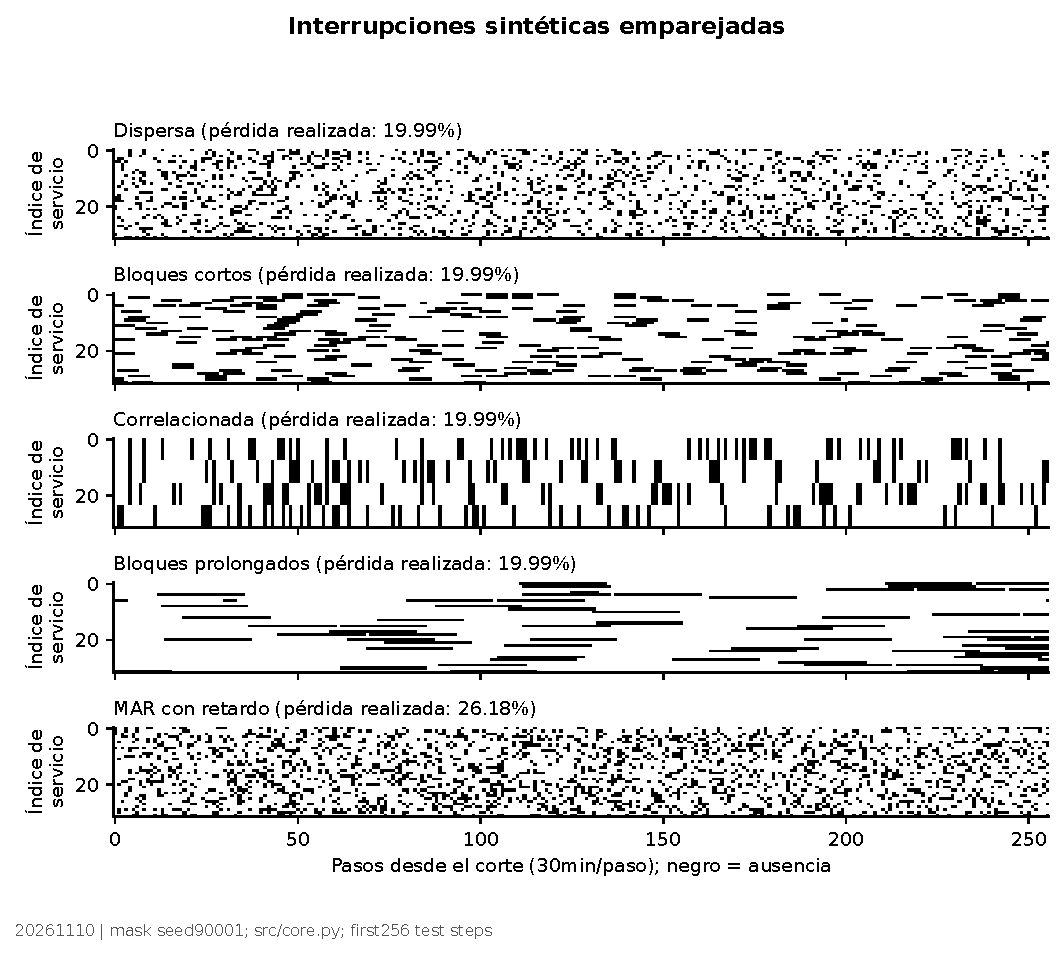
\includegraphics[width=0.68\textwidth]{figuras/es_05_missingness.pdf}
\caption{Máscaras efectivas, semilla 90001 y primeros 256 pasos de prueba. Negro indica ausencia. Correlación y duración son mecanismos impuestos; MAR no afirma 20\% exacto.}\label{fig:masks}\end{figure*}

\subsection{Descomposición histórica y familias compactas}
Para una ventana $ v\in\mathbb R^L $ y una matriz lineal fija de suavizamiento $ S $, DLinear calcula
\begin{align}
\widehat x&=w_t^\top Sv+w_r^\top(I-S)v+b_t+b_r\\
&=[S^\top w_t+(I-S)^\top w_r]^\top v+(b_t+b_r).
\end{align}
E0 utiliza MA25 con extremos replicados incluso cuando L12. El promedio centrado usa posiciones posteriores dentro de la historia, pero ninguna medición futura respecto del origen final. El residual no es una componente estacional demostrada. La transformación fija y la cabeza colapsada representan la misma clase afín; Adam y la regularización pueden seguir trayectorias diferentes. La Fig.~\ref{fig:dlinear} muestra esa distinción.

E1 selecciona ancho 3, 7, 13 o 25. E2 usa una componente exponencial inicializada por $\ell_1=v_1$:
\begin{equation}
\ell_i=\ell_{i-1}+\alpha m_i(v_i-\ell_{i-1}),\qquad r_i=v_i-\ell_i.
\end{equation}
Una imputación no actualiza el nivel como medición nueva. La búsqueda histórica consideró factores fijos 0.1, 0.3, 0.7 y un escalar aprendido mediante sigmoide; las selecciones finales emplearon factores fijos. E3 agrega una proyección sin sesgo de los 36 indicadores de procedencia; E4 proyecta doce edades; E5 combina EMA y ambas cabezas. Sus tamaños con factor fijo son 62, 38 y 74 parámetros frente a 26 de E0/E1/E2. Las cabezas añadidas comienzan en cero. Los indicadores colineales y la edad no son factores informativos ortogonales ni permiten interpretar coeficientes causalmente.

C0--C3 conservan dos cabezas de valor y añaden hasta dos coeficientes escalares:
\begin{equation}
\widehat x_C=\widehat x_{base}+\gamma_p L^{-1}\sum_i(1-m_i)+\gamma_a a_L.
\end{equation}
C0 no añade ninguno, C1 usa fracción ausente, C2 edad final y C3 ambos. Sus tamaños son 26, 27, 27 y 28. Seleccionan MA25, EMA0.3 o EMA0.7. V2 elige una familia por recurso mediante el promedio del mejor MASE de validación de tres ajustes, con desempate por tamaño e identificador. Reutiliza pesos y predicciones; no consulta objetivos futuros ni selecciona por servicio. C3 y V2 no son nombres alternativos de A3.

A0 colapsa las cabezas fijas de DLinear a una proyección afín. A1 agrega $ u=L^{-1}\sum_i(1-m_i)$, A2 la edad logarítmica final $ a=\log(1+\delta_{final})/\log(1+L)$, y A3 ambas:
\begin{equation}
\widehat x_{A3}=w^\top v+b+\gamma u+\eta a.
\end{equation}
Los tamaños son $ L+1,L+2,L+2,L+3$, frente a $2L+2$ de DLinear. A0--A3 inicializan el valor desde las mismas cabezas DLinear sembradas y comienzan los coeficientes adicionales en cero. La equivalencia float 32 inicial se verifica con tolerancias relativa $10^{-5}$ y absoluta $10^{-6}$, no igualdad bit a bit. La edad A no se recorta. Cada familia se selecciona independientemente, por lo que su comparación no mantiene hiperparámetros idénticos. E5 ampliado conserva $\alpha=0.7$ y edad lineal acotada; su descomposición depende de la máscara y queda fuera del colapso fijo. La Fig.~\ref{fig:a3} ilustra A3 y la Fig.~\ref{fig:evolution} sitúa las familias.

\begin{figure*}[!t]\centering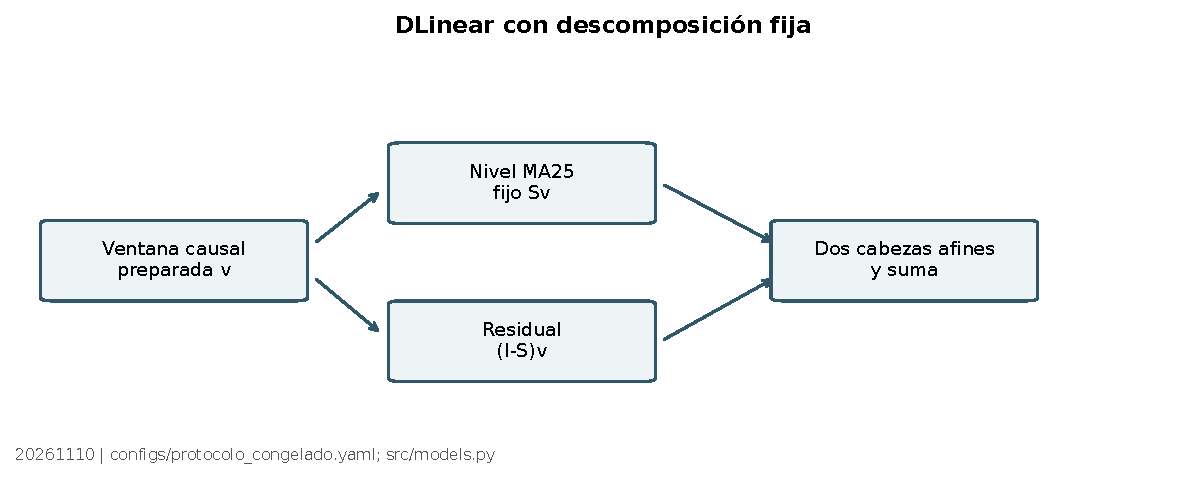
\includegraphics[width=0.79\textwidth]{figuras/es_02_dlinear.pdf}
\caption{Descomposición DLinear fija. Ambas componentes usan la historia disponible. El colapso afín no garantiza trayectoria de optimización idéntica.}\label{fig:dlinear}\end{figure*}

\begin{figure*}[!t]\centering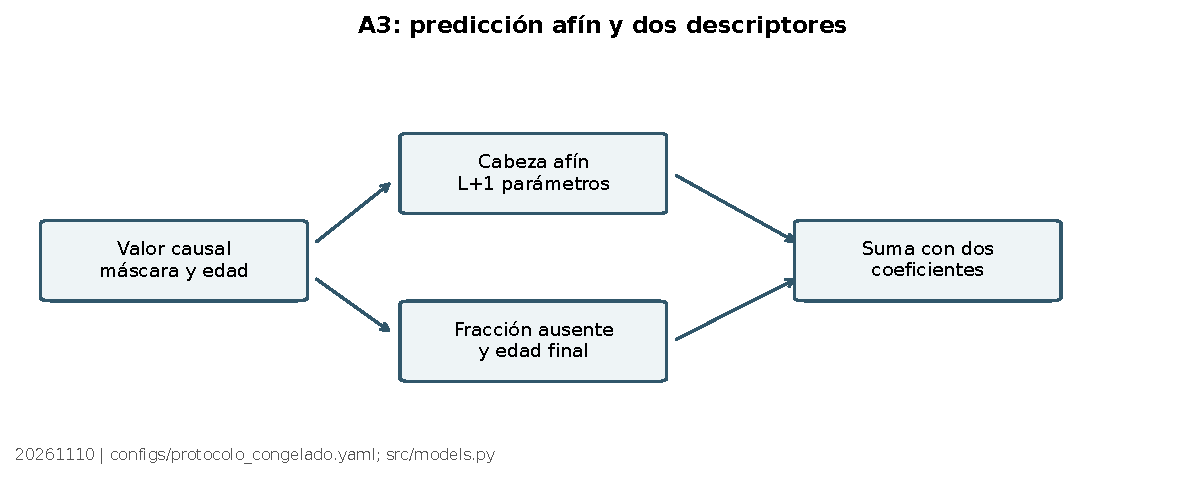
\includegraphics[width=0.79\textwidth]{figuras/es_03_a3.pdf}
\caption{A3 suma fracción ausente y edad logarítmica final a una cabeza afín. L12 requiere 15 parámetros por recurso; los coeficientes adicionales comienzan en cero.}\label{fig:a3}\end{figure*}

\subsection{Comparadores implementados}
Las referencias estadísticas son persistencia, media móvil y suavizamiento exponencial. Los candidatos de media son 1, 3, 6 y 12 pasos incluso con historias mayores. El suavizador actualiza solo con mediciones disponibles y considera $\alpha\in\{0.1, 0.3, 0.7, 0.9\}$. Ridge incluye intercepto no penalizado y $\lambda\in\{0, 10^{-4}, 10^{-2}, 1\}$, con ajuste analítico sobre las diez condiciones preparadas. DLinear, NLinear y las familias A/E comparten pesos entre servicios y separan recursos.

Las GRU ampliadas tienen ancho oculto 12 y nueve canales. La GRU propia repite tres veces el triplete valor/máscara/edad para igualar ancho con la de grafo. Esta última sustituye dos tripletes por agregados entrantes y salientes normalizados por filas. Ambas tienen 841 parámetros. GRU-D adaptada tiene 615, decae la entrada hacia la media normalizada cero, decae el estado y usa una celda con valor e indicador. Estas adaptaciones no reproducen los presupuestos publicados de otras tareas.

PatchTST utiliza código oficial Apache 2.0 en el commit\texttt{204c21efe0b3}, con identificador completo archivado. Emplea un canal, parche 4, paso 2, relleno final, una capa, ancho 16, dos cabezas, ancho interno 32, abandono 0.1 y RevIN afín. Produce un extremo directo. En L12 hay 2499 elementos entrenables y un elemento de escala de atención fijo registrado como parámetro no entrenable. El conteo publicado filtra\texttt{requires\_grad}; los metadatos originales que cuentan todos los tensores se preservan. Estadísticas, matrices de grafo, optimizador y cachés quedan fuera del conteo. El presupuesto pequeño no reproduce las tablas originales de PatchTST. BiTGraph y GinAR permanecen solo en el histórico; TimesNet, iTransformer, TiDE y TimeMixer no se ejecutaron en la ampliación.

\subsection{Selección, ajuste y diseño integrado}
El histórico usa Adam, tasas 0.001/0.003, MSE normalizado, norma de gradiente limitada a uno, lote 16, hasta veinte épocas y paciencia cinco. La asignación de condición por origen y época rota módulo siete. Su búsqueda corta utiliza tres épocas, 512 orígenes de entrenamiento y 32 de validación; el criterio de selección difiere entre variantes originales. Las compactas C comparten seis candidatos de descomposición/tasa por recurso:48 ajustes cortos y 24 finales entre dos recursos y tres semillas. V2 se congela por validación antes de su evaluación, sin eliminar la exposición previa que motivó su diseño.

En la ampliación cada combinación de familia, recurso y configuración recibe cuatro candidatos: tasa $\{0.001, 0.003\}$ por penalización $\{0, 0.001\}$. Se entrenan tres épocas con 512 orígenes fuente y 64 de validación; selecciona MASE de la tercera época sobre diez condiciones. La semilla de búsqueda es 101. El ajuste final utiliza todos los orígenes fuente, Adam, MSE normalizado, recorte 1, máximo 20 épocas, paciencia 5 y mejor checkpoint de validación fuente. La condición por origen rota $(posicion+epoca)\bmod 10$, sin recorrer diez copias completas por época. Validación y evaluación utilizan todas. Igual número de candidatos no equivale a iguales operaciones o tiempo; ridge usa otro presupuesto analítico explícito.

Las semillas principales L12/H1 son 101, 202, 303, 404, 505, 606, 707, 808, 909 y 1010. Son diez ajustes sobre datos fijos, no diez datasets. DLinear, E5, A3, PatchTST y cuatro referencias simples forman el diseño secundario estrella:$ (L,h)=(12, 2),(12, 4),(12, 6),(12, 12),(24, 1),(48, 1)$. Usa tres semillas neuronales y cinco máscaras. A L12 se comparan 30, 60, 120, 180 y 360 minutos; a H1, historias 12, 24 y 48 pasos. No es un factorial completo. Las curvas se reconstruyen sobre la intersección de objetivos válidos y el subconjunto común de semillas/máscaras; no reemplazan el principal completo.

Los hashes del protocolo y código preceden la evaluación destino principal. Cada configuración congela todas sus familias y recursos antes de evaluar. La selección fuente de extensiones ocurre posteriormente en la cola automática sin reajustar a errores destino. Dos enmiendas previas aceleraron GRU-D mediante reproducción CUDA Graph verificada numéricamente y eliminaron acumulación de espacio de trabajo por flujo CUDA. No cambiaron candidatos seleccionados. Se conservaron siete intentos GRU-D fallidos y reintentados. Un ajuste principal de CPU con GRU-D usó microlote 4 tras reducción prescrita. Los checkpoints guardan optimizador, generadores y muestreador al completar épocas; ensayos separados comprobaron reanudación exacta en el mismo entorno.

\begin{table*}[!t]
\caption{Diseño maestro. H se expresa en minutos y L en pasos semihorarios. Los modelos simples tienen un registro seleccionado o ajustado, sin replicación neuronal artificial.}\label{tab:master}
\centering\footnotesize
\begin{tabularx}{\linewidth}{p{.11\linewidth}p{.16\linewidth}p{.28\linewidth}X}
\toprule Fase & Cohorte & Repetición y configuración & Papel y métricas \\\midrule
I & Fuente 28 & E0--E5 y comparadores;3/20;L12/H30 & Exploratorio histórico;MAE/RMSE/MASE \\
II & Fuente 28 & C0--C3 y alias V2;3/20;L12/H30 & Selección por validación e incertidumbre \\
III & Destino 32 & Quince familias;10 semillas neuronales/20 máscaras & Cuatro contrastes principales;resto secundario \\
IV & Destino 32 & Ocho familias;3/5;seis extensiones & H 60/120/180/360 o L24/48;soporte común \\
IV & Alibaba 32 & Catorce familias;pesos congelados;20 máscaras & Doce intervalos calibran y 36 evalúan \\
V & Fuente 28/destino 32 & CUDA B128 histórico y CPU/CUDA B1/B128 ampliado & Parámetros,p 50/p 95,épocas,RSS y asignación separados \\
\bottomrule\end{tabularx}
\end{table*}

\subsection{Métricas y análisis estadístico}
Para $ T $ objetivos válidos de un servicio/recurso,
\begin{align}
MAE&=T^{-1}\sum_t|\widehat y_t-y_t|,\notag\\
RMSE&=\sqrt{T^{-1}\sum_t(\widehat y_t-y_t)^2},\\
d_{s,r}&=|P|^{-1}\sum_{t\in P}|y_{t,s,r}-y_{t-1,s,r}|,\notag\\
MASE&=MAE/d_{s,r}.
\end{align}
$ P $ contiene pares disponibles del prefijo separados 1800 segundos, excluyendo huecos. MAE/RMSE conservan unidades; MASE es adimensional. Un denominador cero produce indefinición, no una constante artificial; todos los observados son positivos. Persistencia de prueba no tiene por qué obtener MASE uno. El RMSE macro promedia raíces por servicio y no una raíz después de agrupar cuadrados. Tampoco pondera por tráfico o magnitud de recursos.

El principal promedia con pesos iguales servicios, seis condiciones originales con pérdidas, veinte máscaras y ajustes sembrados. El caso completo y los tres mecanismos añadidos son secundarios. Para referencia $ B $, se define $\Delta=e_B-e_{A3}$, positivo a favor de A3. La reducción $ R=100(e_B-e_{A3})/e_B $ excluye celdas de referencia cero solo del cálculo porcentual. Se distingue promedio de porcentajes emparejados por celda de porcentaje mediante cociente de medias. En el histórico, la reducción se calcula después de promediar dentro de cada realización de máscara; no es automáticamente el estimando ampliado.

El remuestreo histórico principal toma veinte realizaciones completas con reemplazo 10000 veces, semilla 91001. Se publican por separado intervalos absolutos y porcentuales: los intervalos absolutos antes presentados junto a porcentajes no se reinterpretan como porcentuales. La sensibilidad cruza tres semillas y veinte máscaras preservando emparejamiento. Con tres ajustes su soporte es limitado y no prueba cobertura poblacional ni elimina exploración. No se remuestrean servicios conectados como infraestructuras independientes.

En la ampliación cuatro pruebas exactas bilaterales de signos usan las diez diferencias medias por semilla para A3 frente a DLinear/E5 y dos recursos. Excluyen empates y aplican corrección Holm a cuatro contrastes \cite{holm}. La hipótesis se refiere a $\Pr(\Delta_{semilla}>0)=1/2$ condicionada al modelo de ajustes, no a que la diferencia media aritmética poblacional sea cero. La semilla 101 interviene también en búsqueda fuente. Una sensibilidad declarada antes de inspeccionar métricas destino la elimina y ajusta separadamente nueve semillas; es diagnóstica y no sustituye el principal.

Los intervalos ampliados usan 2000 réplicas cruzadas de semillas, máscaras y bloques temporales circulares, semilla 61110. El bloque principal es 48 pasos, con sensibilidad 24/96. Los servicios permanecen juntos. La interpretación está condicionada al período, servicios y configuraciones seleccionadas; requiere aproximaciones de dependencia local y estacionariedad. No son intervalos de infraestructura poblacional ni de predicción. Se añaden efectos por servicio, desviaciones entre medias de semillas/máscaras y resúmenes descriptivos por bloques no solapados de 48 orígenes. Los secundarios y externos carecen de afirmaciones confirmatorias.

El tamaño cuenta escalares entrenables. Los percentiles de latencia son cuantiles empíricos de llamadas cronometradas por dispositivo/lote. El rendimiento depende del número de orígenes y servicios por llamada. La duración de ajuste incluye épocas completadas y validación bajo el alcance registrado; ni parámetros ni latencia miden energía o coste monetario.

\subsection{Entorno, ejecución y medición computacional}
Se usa Docker con Debian GNU/Linux 13, Python 3.12, PyTorch 2.9.0+cu128, Intel Core i 5-11300H de cuatro núcleos/ocho hilos, aproximadamente 24~GB RAM y RTX 3050 Laptop de 4~GB nominales, controlador 550.163.01. El entrenamiento es float 32, dos hilos CPU, lote efectivo 16 y microlote 8 con acumulación. BatchNorm de PatchTST recibe el microlote, no un lote físico 16. Se activan algoritmos deterministas y desactiva TF 32. Una cola GPU del proyecto convive con aplicaciones del usuario. Los monitores registran memoria, temperatura e intercambio y pueden pausar el ejecutor del proyecto.

El benchmark histórico usa proceso separado por modelo, B128, diez calentamientos y cien repeticiones distribuidas en cinco bloques, con CUDA sincronizada y ejecución directa float 32. Las salidas se comparan con predicciones archivadas. Se conservan p 50/p 95, RSS y asignación CUDA; los tiempos de ajuste se acompañan de épocas. La reanudación histórica tras apagado verificó 78 checkpoints completos sin cambios. Un ensayo separado de interrupción reprodujo pesos y métricas: valida el mecanismo, no una trayectoria contrafactual del equipo.

Después del ajuste ampliado, CPU y CUDA se miden secuencialmente en B1 y B128, 32 servicios y tensores residentes. Veinte calentamientos preceden cien llamadas por configuración, con sincronización CUDA y orden aleatorizado fijo. La reproducción CUDA de GRU-D se distingue de ejecución directa y excluye captura inicial de la latencia. Las sumas de épocas incluyen validación y captura inicial, pero excluyen búsqueda, escritura de checkpoints e intentos fallidos incompletos. La coexistencia con preparación de datos y aplicaciones limita atribuir diferencias solo a la arquitectura. RSS de proceso, asignación PyTorch y memoria GPU del sistema tienen alcances diferentes. No se instrumentó energía fiable y no se estiman beneficios operativos.
